

\begin{flushleft}
	
	\begin{itemize}
		\item Boolean is datatype for logical values. 
		\item Boolean is return by all relational operators.

	\end{itemize}
		
		\tabletwo{
			\hline
			Size & \textbf{1 byte (8 bits)}. The actual memory usage may depend on JVM implementation. \\
			\hline
			Value & true, false \\
			\hline
		}

		\begin{figure}[h!]
			\centering
			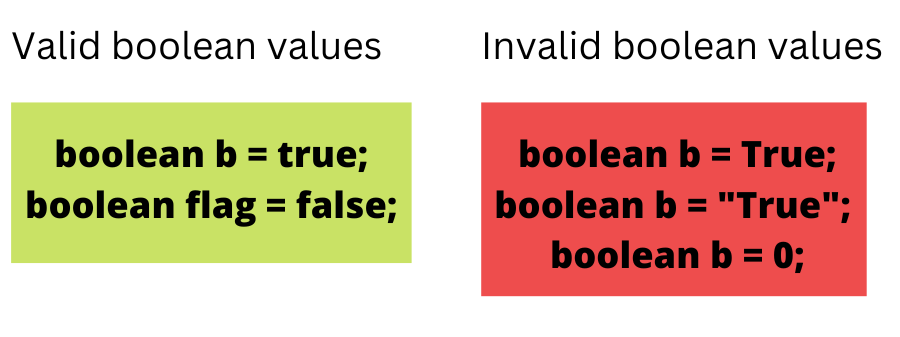
\includegraphics[scale=.35]{content/chapter2/images/boolean.png}
		\end{figure}		
				
		\noteblock{
			\begin{itemize}
				\item The values of true and false do not convert into any numerical representation. 
				\item The true literal in Java does not equal 1, nor does the false literal equal 0. 
			\end{itemize}
		}
		\begin{figure}[h!]
			\centering
			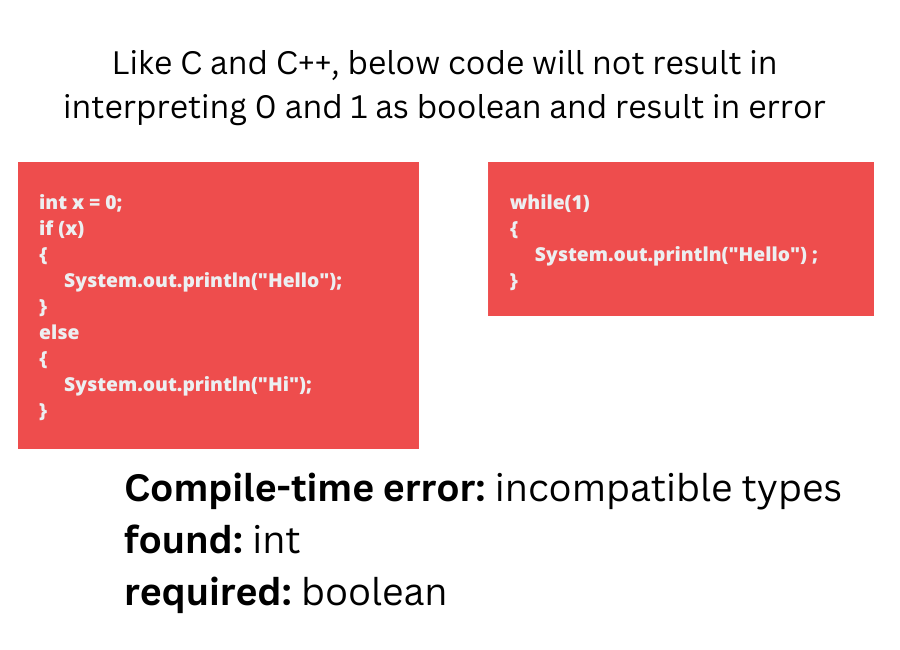
\includegraphics[scale=.45]{content/chapter2/images/bool.png}
		\end{figure}		
				
		
		

	
\end{flushleft}

\newpage

